\section{Broader tests of the frozen application}
\label{sec:extended-coverage}
The earlier gains concern selected graph structures and target patterns. We now keep the deployed models and all decision rules fixed and test a wider set of physical inputs. The expanded test defines 84 native family requests at one through twelve loops. 29 requests complete all methods and exact checks, while 36 exceed the current 31-index interface limit. The remaining requests retain their recorded failures. The separate analytic test verifies 24 scalar massless two-point batches, covering every loop order from one through twelve at both rational and symbolic momentum. A loop label alone therefore does not specify the demonstrated scope: the graph, masses, external momenta, target powers, and method also matter.

\subsection{Physical inputs and checks}
The native grid contains one-mass and fully massive vacuum families, massless and massive two-point families, four-point ladders, and boxes with bubble subgraphs. It also contains nonplanar boxes, pentagons, and boxes with one external virtuality. Rational profiles differ from those in the preceding studies. Selected low-loop cases keep the independent masses and momentum invariants symbolic. Appendix~\ref{app:extended-coverage} gives the target sets and parameter choices, using the previously defined denominators.

Each eligible request first runs Kira with expanded seeds and no preferred master basis. A second reduction changes the integral ordering and increases the numerator bound, then checks every coefficient in the discovered basis. This agreement tests stability within those two seed regions; it does not prove that every surviving master is independent under all possible IBP identities. The reference stage records 13 time-limit failures and 6 Kira allocation failures. The latter occur during topology preparation under the address-space cap, before a learned reduction decision is tested. These failures therefore identify preparation and resource limits, rather than model prediction errors. The three timed methods then receive that common basis. Kira generates their equations and performs the exact reduction, as in its standard reduction procedure~\cite{KiraOriginal,Kira3}.

The native control disables learned choices and uses the current exact implementation with fixed bounds. The previous and selected applications use their unchanged published policies. Each run starts a fresh process, and its time includes imports, input preparation, model loading, equation generation, algebra, coefficient checks, retries, and process exit. Every method loads the common application modules, including the native and direct-formula controls. These are complete times for the same interface, rather than timings of the Kira executable alone. The comparison includes costs that can matter for small requests. Master discovery and the independent reference calculation remain separate. Three repetitions rotate method order on the same worker for each case. Each native attempt has a 30-second budget, a 32 MiB temporary-storage limit, and the existing memory guard. The runner reserves ten seconds for completion and cleanup, leaving at most twenty seconds for the Kira process. A failure stops further repetitions of that method, and remains in the coverage count.

\begin{table}[!htbp]\centering\small
\caption{Outcomes for the complete predefined native grid. Rejected inputs have no timed Kira reduction.}
\label{tab:extended-coverage}
\begin{tabular}{@{}lr@{}}\toprule
Outcome & Requests\\\midrule
All methods verified & 29\\
Reference limit or failure & 14\\
Reference check failure & 5\\
Input index limit & 36\\
\bottomrule\end{tabular}\end{table}

\begin{table}[!htbp]\centering\small
\caption{Results by loop order. Native verified counts require all methods and reference checks. A dash means no matched nontrivial native timing comparison. Analytic checks cover the stated scalar massless two-point family.}
\label{tab:extended-loops}
\begin{tabular}{@{}rrrrr@{}}\toprule
Loops & Native verified/requested & Matched & Time ratio & Analytic passed\\\midrule
1 & 12/12 & 12 & 0.988 & 2/2\\
2 & 10/12 & 10 & 1.020 & 2/2\\
3 & 4/6 & 4 & 0.918 & 2/2\\
4 & 3/6 & 3 & 1.038 & 2/2\\
5 & 0/6 & 0 & -- & 2/2\\
6 & 0/6 & 0 & -- & 2/2\\
7 & 0/6 & 0 & -- & 2/2\\
8 & 0/6 & 0 & -- & 2/2\\
9 & 0/6 & 0 & -- & 2/2\\
10 & 0/6 & 0 & -- & 2/2\\
11 & 0/6 & 0 & -- & 2/2\\
12 & 0/6 & 0 & -- & 2/2\\
\bottomrule\end{tabular}\end{table}

\subsection{Complete application times}
The matched nontrivial set contains 29 requests for which all three repetitions of all methods pass the exact coefficient checks. A nontrivial reduction has at least one nonzero target expression beyond the unchanged target itself. We report the sum of per-request median times, using the definition in Appendix~\ref{app:coverage}. Identity-only answers and failed requests do not enter this time ratio. The two single-target rank-three box requests lack fully checked references under the common limits and therefore supply no new timing comparison for the learned sparse-seed route.

\begin{table}[!htbp]\centering\small
\caption{Complete times on the matched nontrivial requests. Ratios compare selected time with native time; a value below one means less time.}
\label{tab:extended-times}
\begin{tabular}{@{}lrrrr@{}}\toprule
Family & Requests & Native (s) & Selected (s) & Ratio\\\midrule
bubble box & 1 & 1.077 & 1.295 & 1.202\\
ladder & 4 & 6.786 & 6.755 & 0.995\\
nonplanar box & 2 & 11.028 & 11.246 & 1.020\\
one mass box & 2 & 2.228 & 2.386 & 1.071\\
pentagon & 2 & 2.915 & 2.582 & 0.886\\
propagator massive & 6 & 9.798 & 9.985 & 1.019\\
propagator massless & 4 & 4.436 & 4.155 & 0.937\\
vacuum all mass & 3 & 5.081 & 5.076 & 0.999\\
vacuum one mass & 5 & 5.548 & 5.550 & 1.000\\
\midrule
All matched & 29 & 48.896 & 49.030 & 1.003\\
\bottomrule\end{tabular}\end{table}

The previous application takes 48.136 seconds on the same set. The selected application's total differs from the native total by 0.3\%, and the timing interval includes equal time. The selected-to-native time ratio is 1.003, with a paired-repetition resampling interval [0.968, 1.073]. The interval describes timing variation for these fixed cases; it does not estimate coverage of all integral families. Reference discovery takes a further 71.653 seconds, and its independent check takes 117.521 seconds. Adding the same measured discovery work to each method gives 120.549 seconds for the native control and 120.684 seconds for the selected application. This last comparison includes discovery once per request and does not represent a learned master-discovery method.

These are comparisons of complete deployed configurations. Outside the fitted domain, the selected application can take an exact analytic route or fall back to native choices. In the matched set, 2 cases use the analytic formula and the remaining cases use native choices. No matched case activates a learned seed, batch, or equation decision. The frozen domain checks and validation gates determine these routes. This comparison therefore checks application coverage and fallback behavior, and its time difference supplies no evidence of a learned gain on these new targets. The earlier matched filter and sparse-seed controls remain the evidence for isolated learned gains.

\begin{figure}[!htbp]\centering
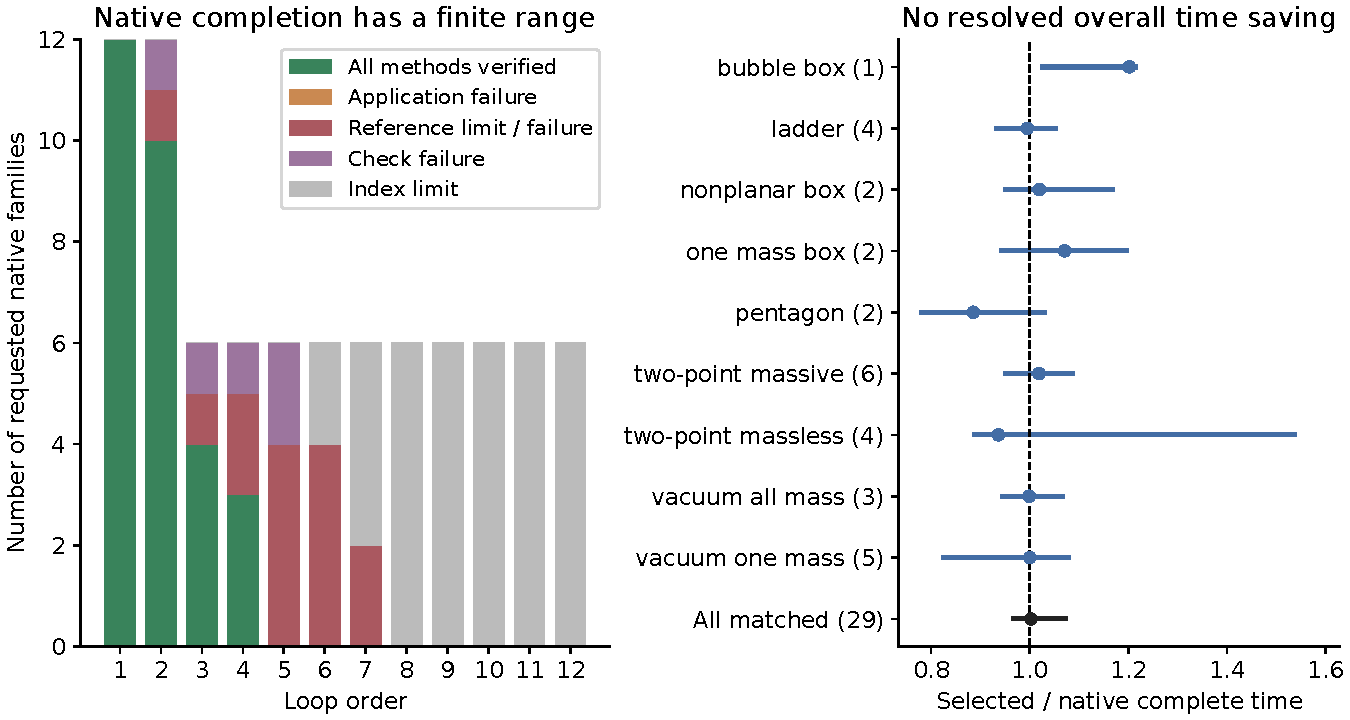
\includegraphics[width=\linewidth]{paper_figures/extended_coverage.pdf}
\caption{Left: every requested native family remains in the coverage count, including failures and input limits. Right: time-ratio points and paired-repetition intervals use only matched nontrivial cases, with case counts in parentheses. The dashed line marks equal time. The panels distinguish whether a calculation finishes from how long a completed calculation takes.}
\label{fig:extended-coverage}
\end{figure}\FloatBarrier

\subsection{Exact checks at every studied loop order}
The analytic test uses the scalar massless two-point family of Appendix~\ref{app:banana} and four target patterns at each loop order, with either a new rational value of $p^2$ or symbolic $p^2$. An independently implemented recurrence raises one propagator power at a time and checks each exact coefficient returned by the frozen application. Appendix~\ref{app:extended-coverage} derives this recurrence. All 24 batches pass, with four targets per batch and three repetitions of the direct formula, previous application, and selected application.

These inputs contain only the physical denominators. The analytic formula needs no auxiliary numerator coordinates, while general native IBP generation uses a complete scalar-product basis. For that complete representation, the current interface reaches its index limit at lower loop order. The twelve-loop analytic checks therefore verify the stated scalar family and exact route; they do not establish general native twelve-loop reductions or learned speedups at twelve loops.

\subsection{Reuse on the additional physical inputs}
Four base requests are fixed before testing: planar and nonplanar two-loop rank-three boxes, a one-loop ladder, and a two-loop massless two-point family. Each sequence changes all external scalar products by factors $1$, $3/2$, and $2$. Independent native references check each scale. The application can reuse only graph signatures already supported by the frozen scaling rule. Every measured sequence includes its first reduction and three repetitions rotate method order.

2 of the four sequences complete every paired method. Their summed median times are 4.601 seconds for the previous application, 4.581 seconds for the selected application without reuse, and 4.546 seconds with reuse. The ratio of selected reuse time to previous time is 0.988. The completed sequences record 0 reused outputs across the three repetitions. The retained records include any sequence that fails to obtain a checked reference. The completed sequences have no reuse hits because their graphs lie outside the current scale-cache domain. The two rank-three box sequences lack checked references within the limits, so this extension provides no new measurement of the reuse benefit. It checks sequence processing and the domain rules without new model training or a changed policy.

The full extension retains 495 successful measured calls and 0 failed measured calls, excluding the independent native references. The exact checks compare 6399 coefficient pairs. The result states where the existing method works under the specified limits. General reductions for every topology and arbitrary loop order remain unverified.
